\setcounter{page}{1}
\pagenumbering{Roman}

\section{Appendix}

% Listado de apartados que son demasiado extensos para incluir en la memoria y tienen un carácter autocontenido (por ejemplo, manuales de usuario, manuales de instalación, etc.)
 
% Dependiendo del tipo de trabajo, es posible que no sea necesario añadir ningún anexo.



% \subsection*{Anexo A: Motivos de RNA empleados en este trabajo (en formato \texttt{.fasta})}\label{anexo_A}
% \addcontentsline{toc}{subsection}{Anexo A: Motivos de RNA empleados en este trabajo (en formato \texttt{.fasta})}

% \lstinputlisting{assets/motifs.fasta}

% \subsection*{Anexo B: Motivos de RNA junto a su alineamiento con la secuencia original y estructura secundaria}\label{anexo_B}
% \addcontentsline{toc}{subsection}{Anexo B: Motivos de RNA junto a su alineamiento con la secuencia original y estructura secundaria}

% \lstinputlisting[basicstyle=\tiny]{assets/dataset.tsv}

% \subsection*{Anexo C: Script de \texttt{Python} para el tratamiento de los motivos de RNA}\label{anexo_C}
% \addcontentsline{toc}{subsection}{Anexo C: Script de \texttt{Python} para el tratamiento de los motivos de RNA}

% \lstinputlisting[language=Python]{assets/motifs_treatment.py}

% \subsection*{Anexo D: Conformaciones 3D de los motivos de RNA}\label{anexo_D}
% \addcontentsline{toc}{subsection}{Anexo D: Conformaciones 3D de los motivos de RNA}

% \begin{center}
%     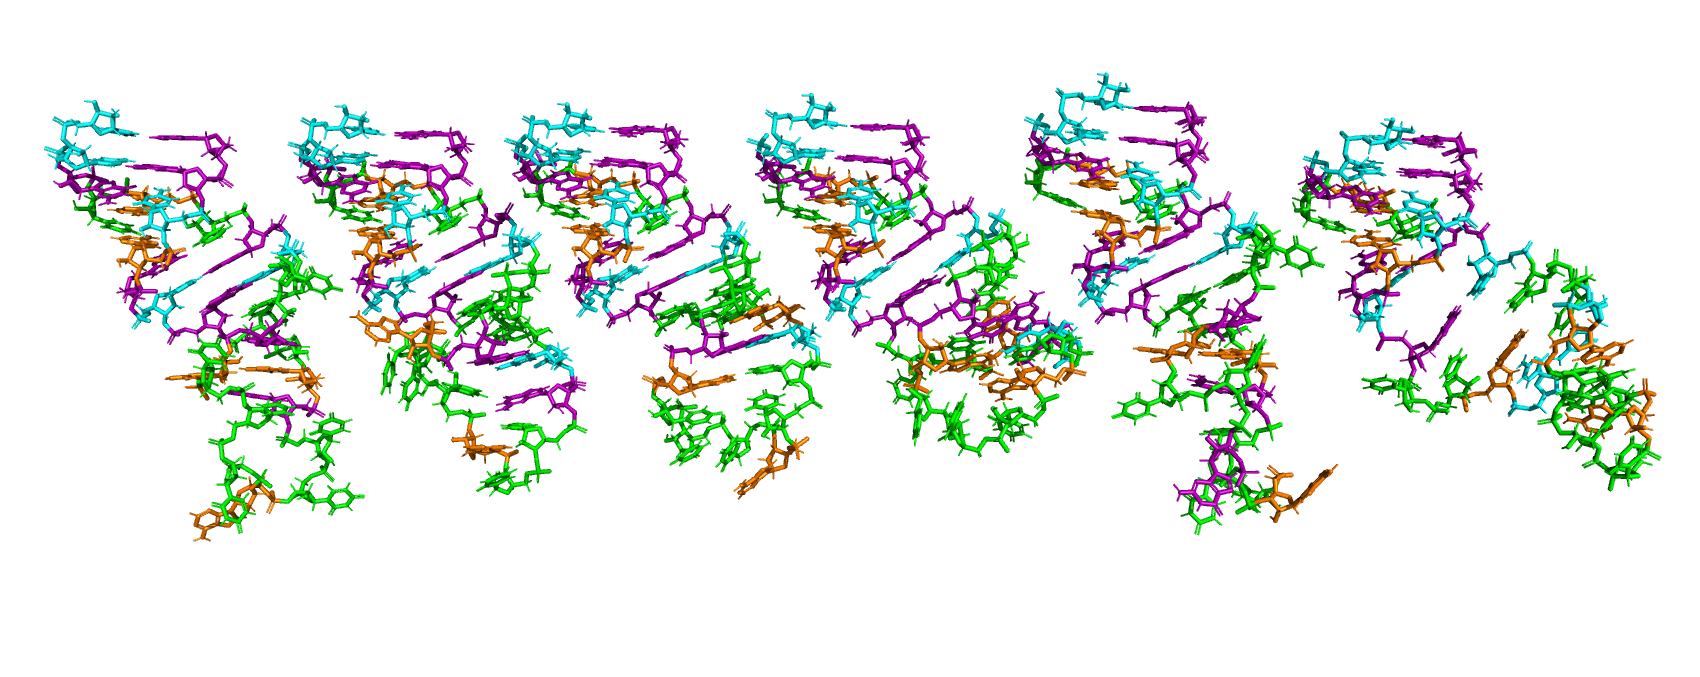
\includegraphics[width=\linewidth]{assets/RNAs.png}
% \end{center}

% De izquierda a derecha: el motivo de RNA original seguido de los 5 mutantes. Los colores representan las bases nucleotídicas: naranja es Adenina, violeta es Guanina, cian es Citosina y verde es Uracilo. Visualizado con \href{https://pymol.org/2/}{\texttt{Pymol}}.

% \subsection*{Anexo G: Visualización de la estructura 3D de los ácidos grasos}\label{anexo_G}
% \addcontentsline{toc}{subsection}{Anexo G: Visualización de la estructura 3D de los ácidos grasos}

% \begin{center}
%     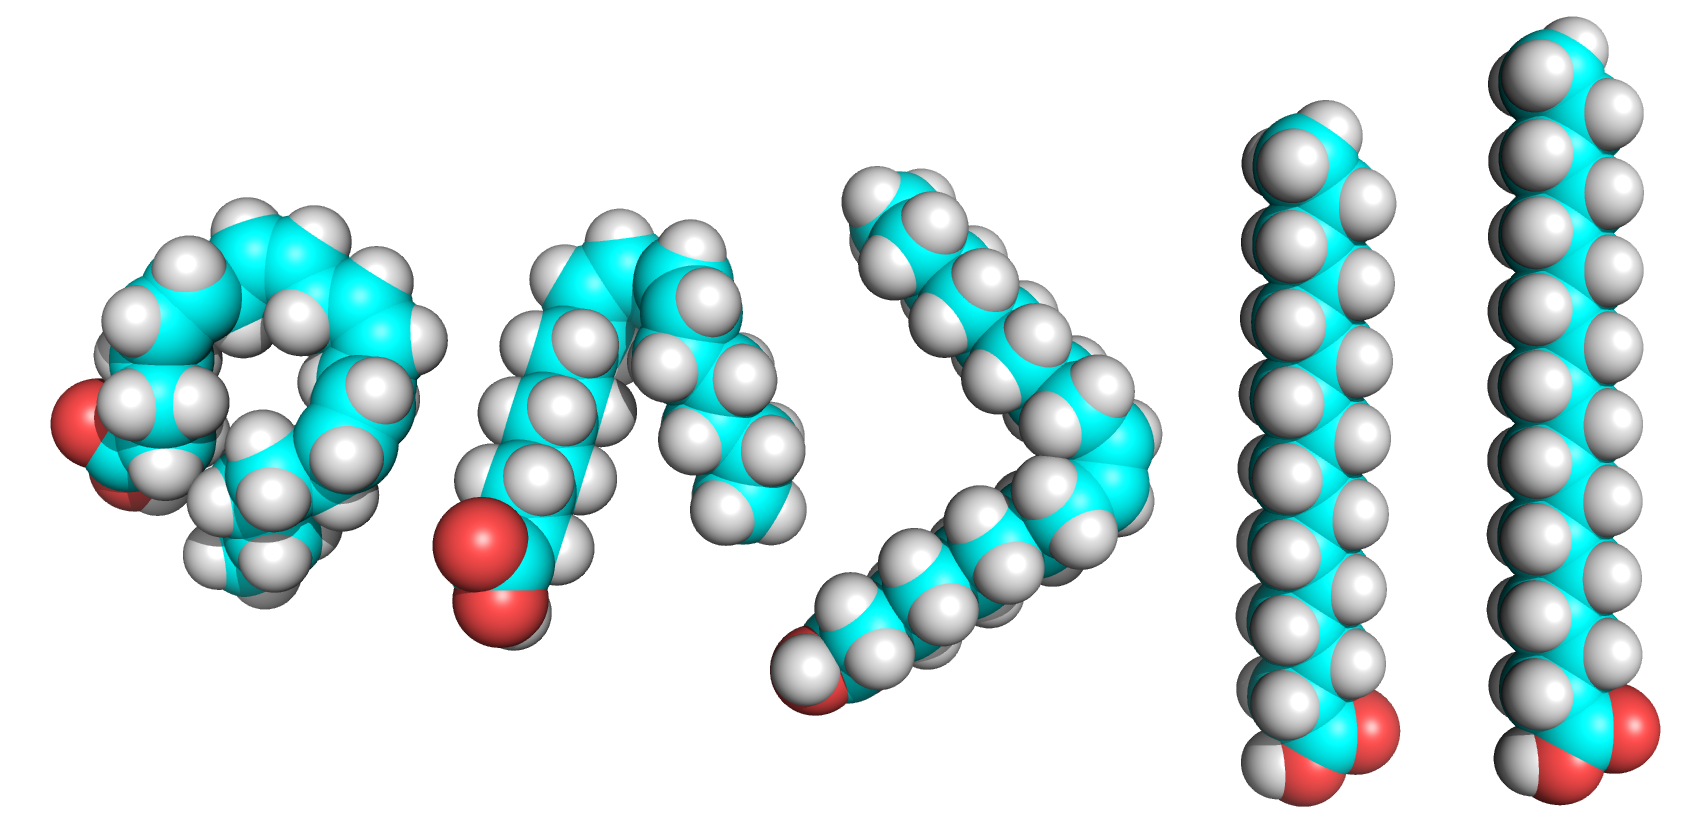
\includegraphics[width=0.633\linewidth]{assets/fatty_acids.png}
% \end{center}

% Visualización en 3D de los ácidos grasos seleccionados. De izquierda a derecha: ácido araquidónico, ácido linoleico, ácido oleico, ácido palmítico y ácido esteárico. Los colores representan los átomos: cian es Carbono, rojo es Oxígeno y blanco es Hidrógeno. Visualizado con \href{https://pymol.org/2/}{\texttt{Pymol}}.

% \subsection*{Anexo A: Script de \texttt{Python} para la mitigación de los tags \texttt{R} en los ficheros \texttt{.pdb} de los RNAs}\label{anexo_A}
% \addcontentsline{toc}{subsection}{Anexo A: Script de \texttt{Python} para la mitigación de los tags \texttt{R} en los ficheros \texttt{.pdb} de los RNAs}

% \lstinputlisting[language=Python]{assets/manipulateRNA.py}

% \subsection*{Anexo B: Script de \texttt{Python} para la recuperación de los tags \texttt{R} en los ficheros \texttt{.pdb} de los RNAs}\label{anexo_B}
% \addcontentsline{toc}{subsection}{Anexo B: Script de \texttt{Python} para la recuperación de los tags \texttt{R} en los ficheros \texttt{.pdb} de los RNAs}

% \lstinputlisting[language=Python]{assets/manipulateRNAagain.py}

% \subsection*{Anexo C: Script de \texttt{Python} para eliminar grupos hydroxilos en los extremos 3' y 5'}\label{anexo_C}
% \addcontentsline{toc}{subsection}{Anexo C: Script de \texttt{Python} para eliminar grupos hydroxilos en los extremos 3' y 5'}

% \lstinputlisting[language=Python]{assets/removeEnds.py}

% \subsection*{Anexo D: Script de \texttt{Python} para re-etiquetar correctamente los resíduos de Histidina}\label{anexo_D}
% \addcontentsline{toc}{subsection}{Anexo D: Script de \texttt{Python} para re-etiquetar correctamente los resíduos de Histidina}

% \lstinputlisting[language=Python]{assets/fixHIS.py}

% \subsection*{Anexo E: Visualización de los 10 mejores modelos de docking entre MSI-1 y el RNA original (\textit{wild type})}\label{anexo_E}
% \addcontentsline{toc}{subsection}{Anexo E: Visualización de los 10 mejores modelos de docking entre MSI-1 y el RNA original (\textit{wild type})}

% \begin{center}
%     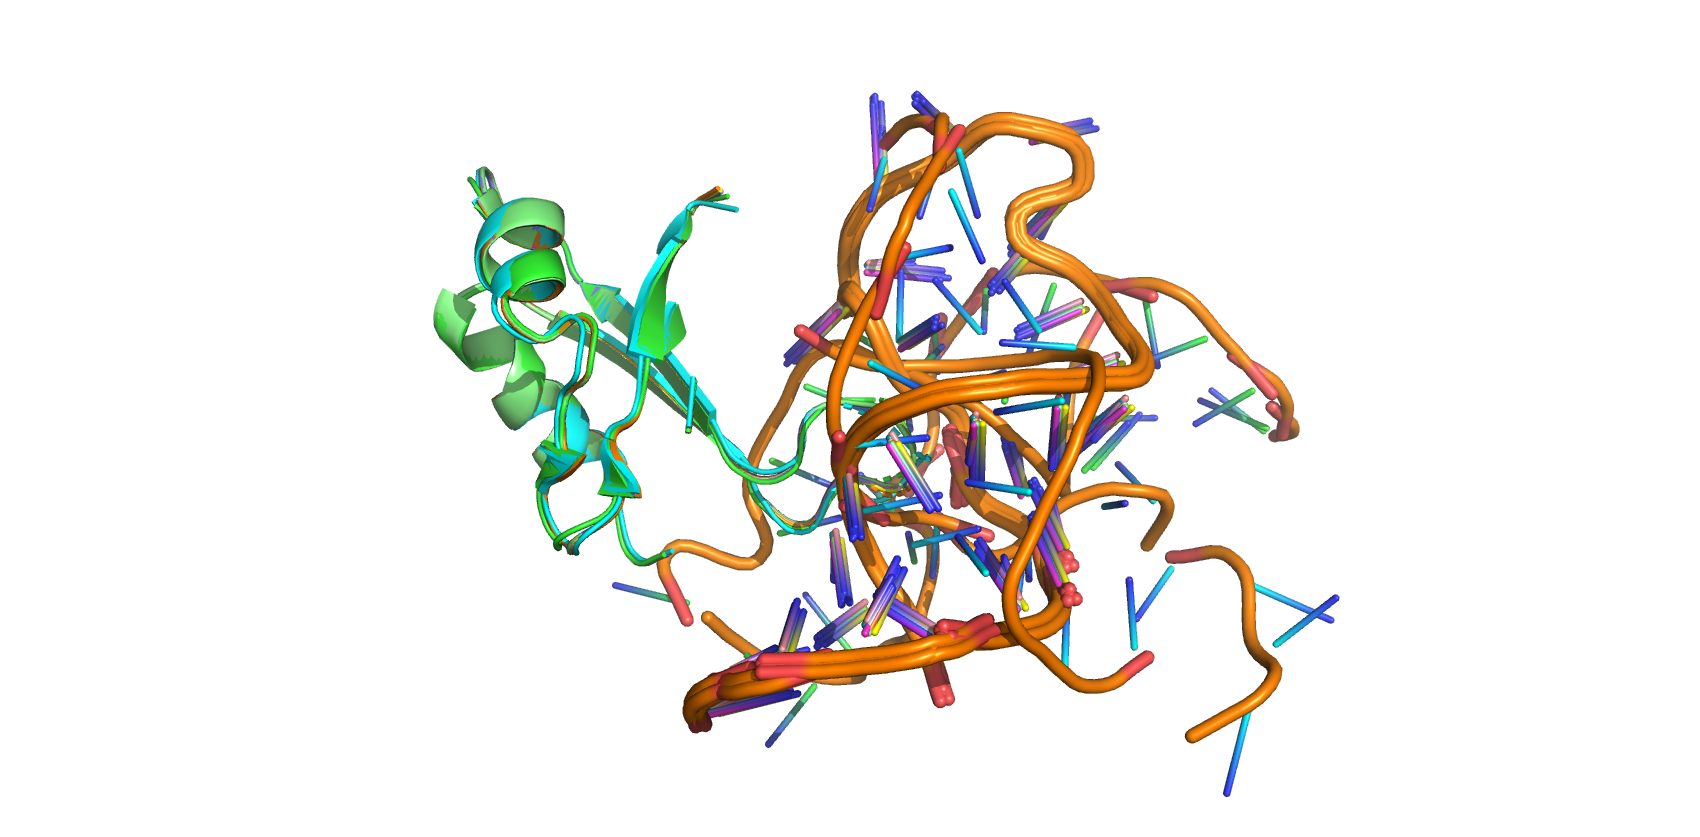
\includegraphics[width=\linewidth]{assets/RMM1_orig_ALL.png}
% \end{center}

% Podemos observar que los modelos difieren entre sí. En los subsiguientes anexos, estos modelos serán desglosados. Visualizado con \href{https://pymol.org/2/}{\texttt{Pymol}}.

% \subsection*{Anexo F: Visualización del mejor modelo de docking entre MSI-1 y el RNA original (\textit{wild type})}\label{anexo_F}
% \addcontentsline{toc}{subsection}{Anexo F: Visualización del mejor modelo de docking entre MSI-1 y el RNA original (\textit{wild type})}

% \begin{center}
%     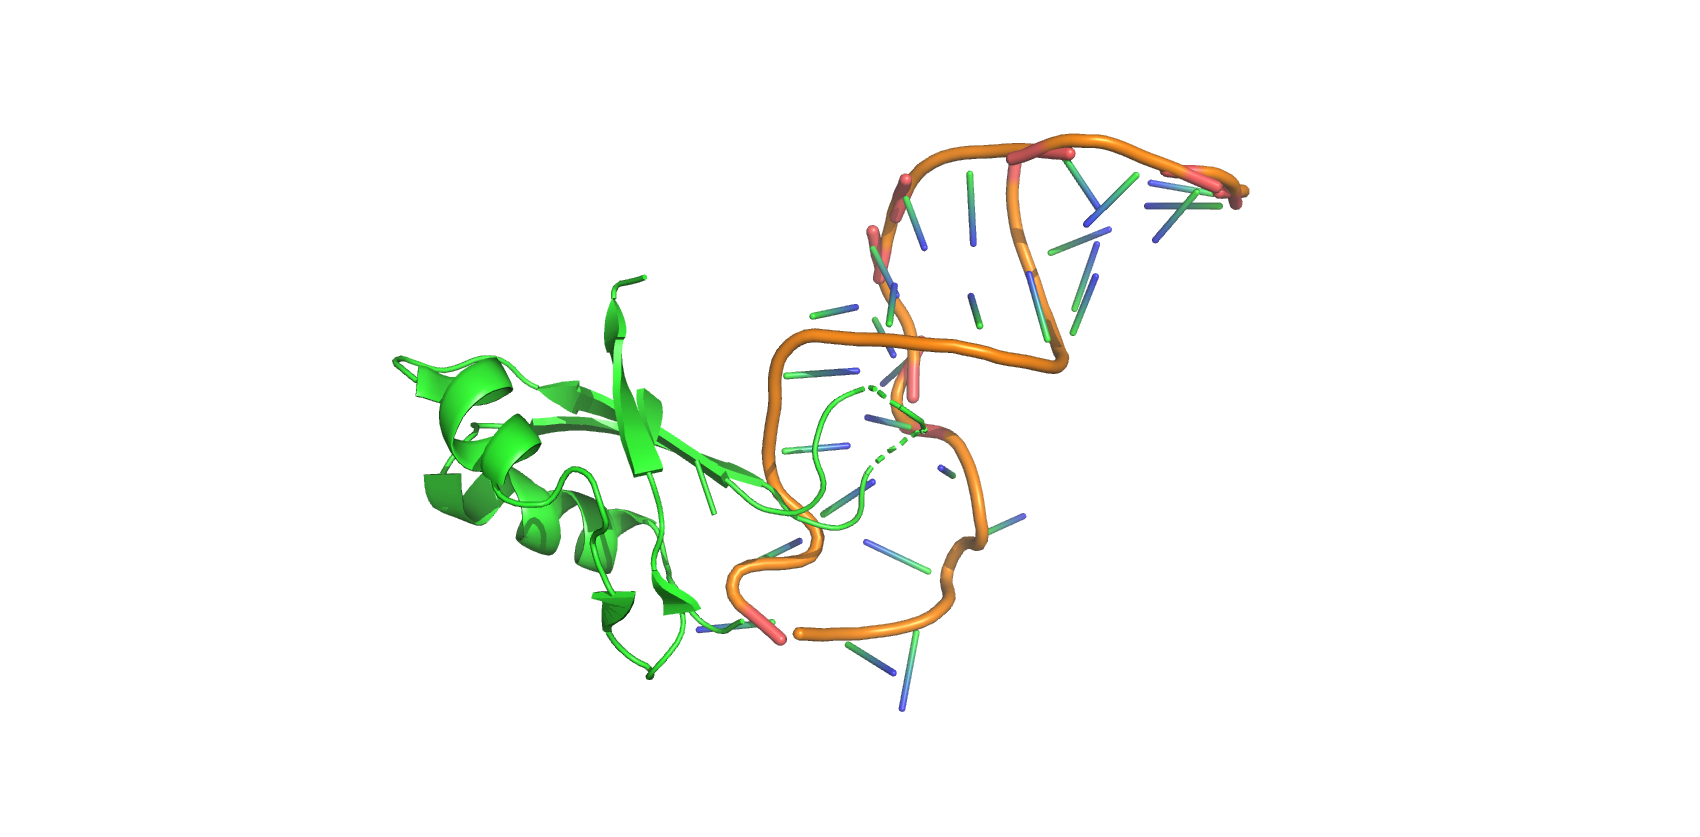
\includegraphics[width=\linewidth]{assets/RMM1_orig_top0.png}
% \end{center}

% Visualizado con \href{https://pymol.org/2/}{\texttt{Pymol}}.

% \subsection*{Anexo G: Visualización del segundo mejor modelo de docking entre MSI-1 y el RNA original (\textit{wild type})}\label{anexo_G}
% \addcontentsline{toc}{subsection}{Anexo G: Visualización del segundo mejor modelo de docking entre MSI-1 y el RNA original (\textit{wild type})}

% \begin{center}
%     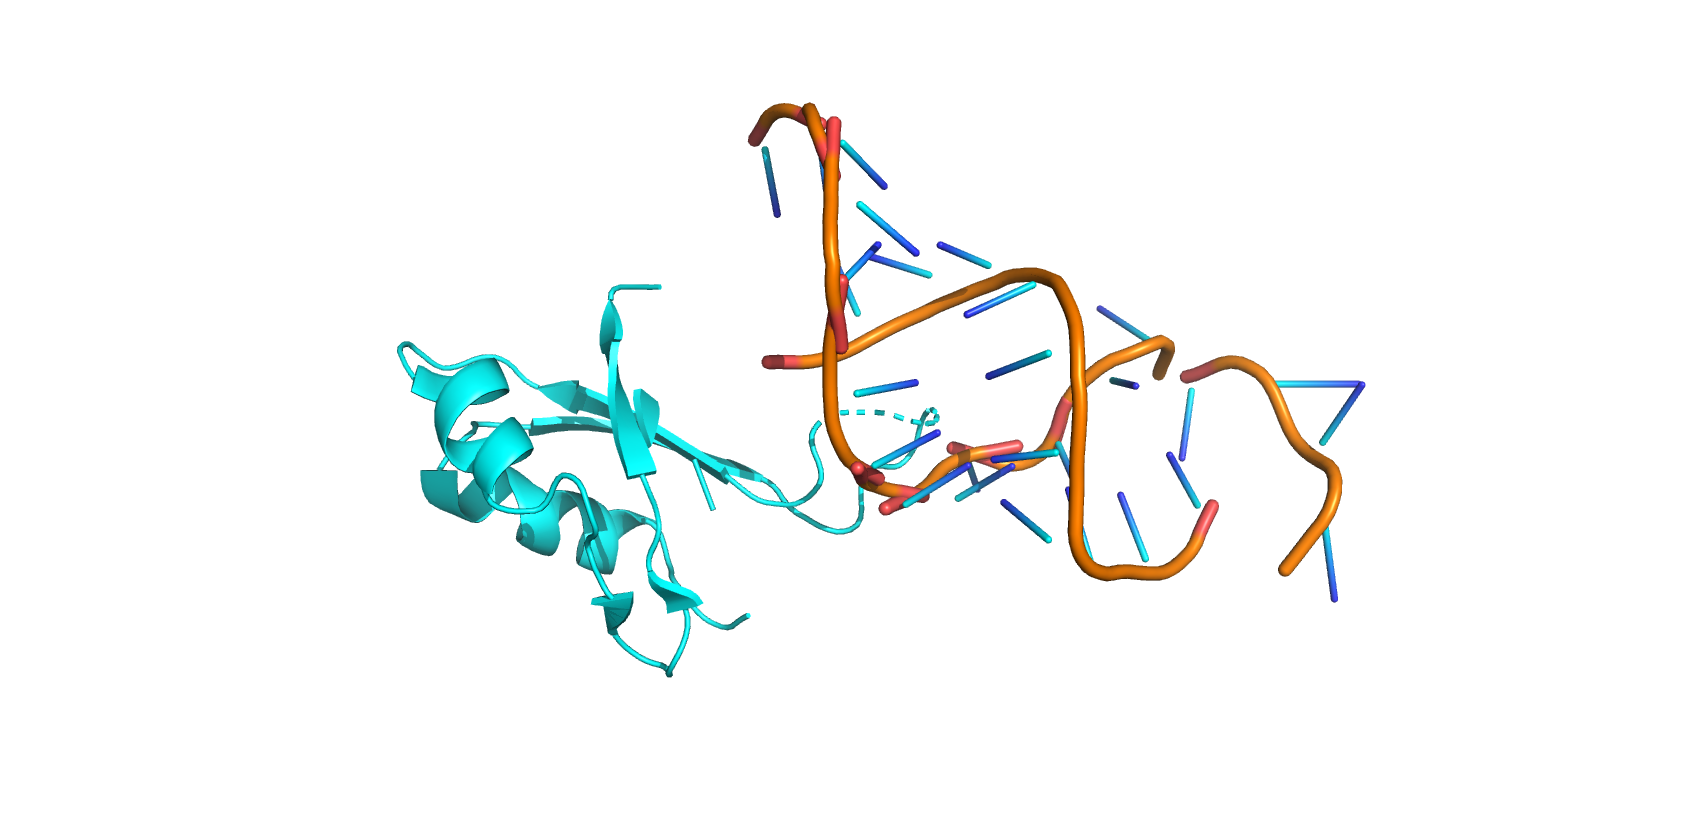
\includegraphics[width=\linewidth]{assets/RMM1_orig_top1.png}
% \end{center}

% Visualizado con \href{https://pymol.org/2/}{\texttt{Pymol}}.

% \subsection*{Anexo H: Visualización del tercer al décimo mejores modelos de docking entre MSI-1 y el RNA original (\textit{wild type})}\label{anexo_H}
% \addcontentsline{toc}{subsection}{Anexo H: Visualización del tercer al décimo mejores modelos de docking entre MSI-1 y el RNA original (\textit{wild type})}

% \begin{center}
%     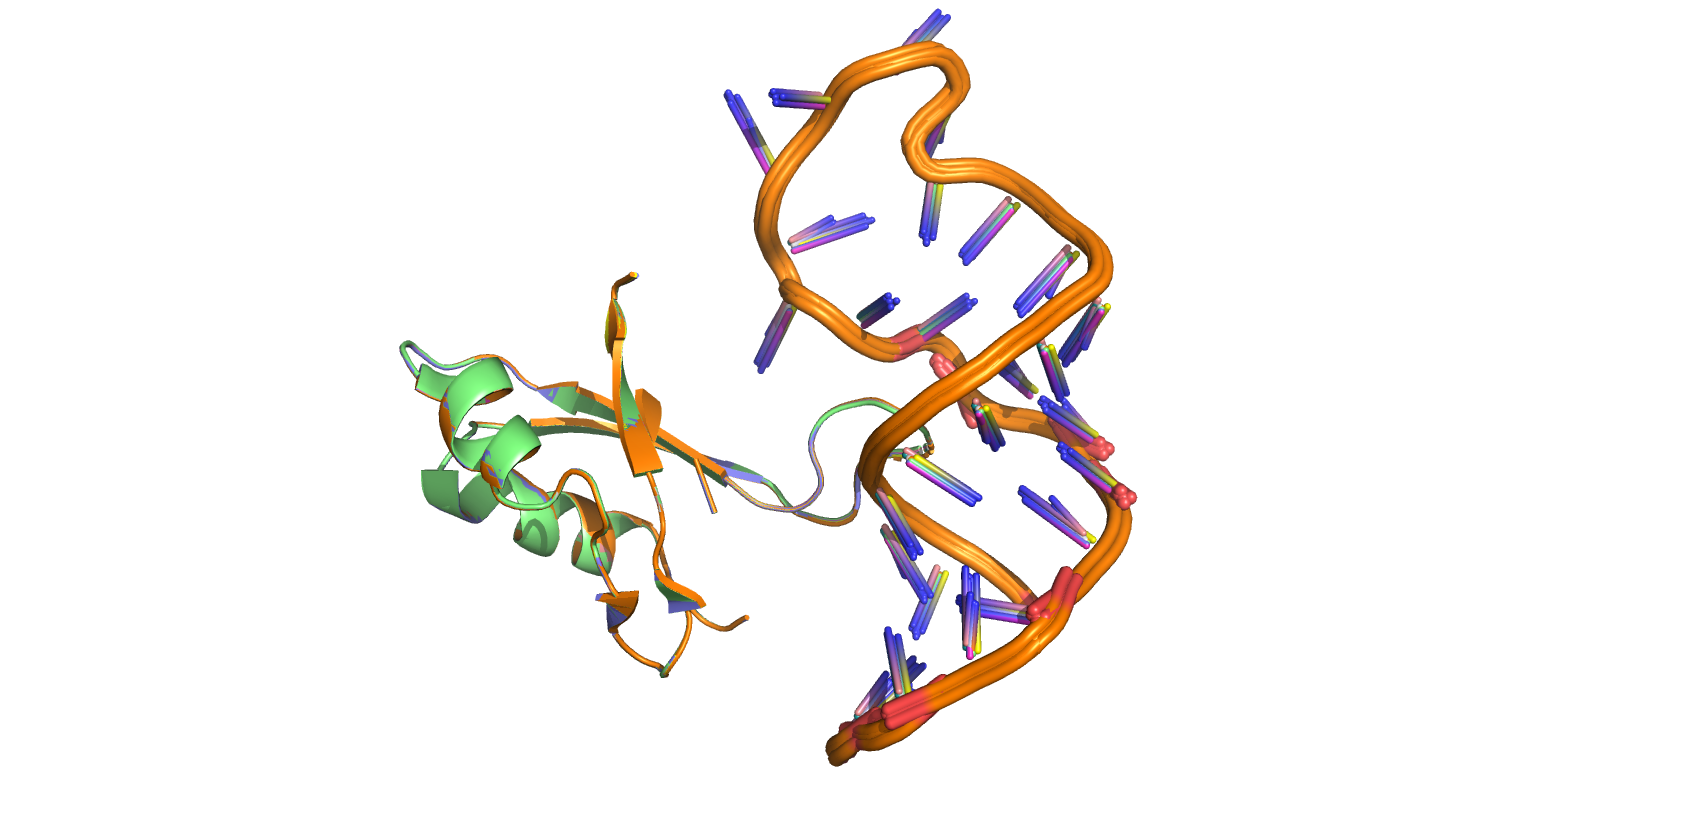
\includegraphics[width=\linewidth]{assets/RMM1_orig_2to8.png}
% \end{center}

% Podemos observar que estos modelos son casi equivalentes. Visualizado con \href{https://pymol.org/2/}{\texttt{Pymol}}.

% \subsection*{Anexo I: Visualización de los 10 mejores modelos de docking entre MSI-1 y el RNA mutante 1}\label{anexo_I}
% \addcontentsline{toc}{subsection}{Anexo I: Visualización de los 10 mejores modelos de docking entre MSI-1 y el RNA mutante 1}

% \begin{center}
%     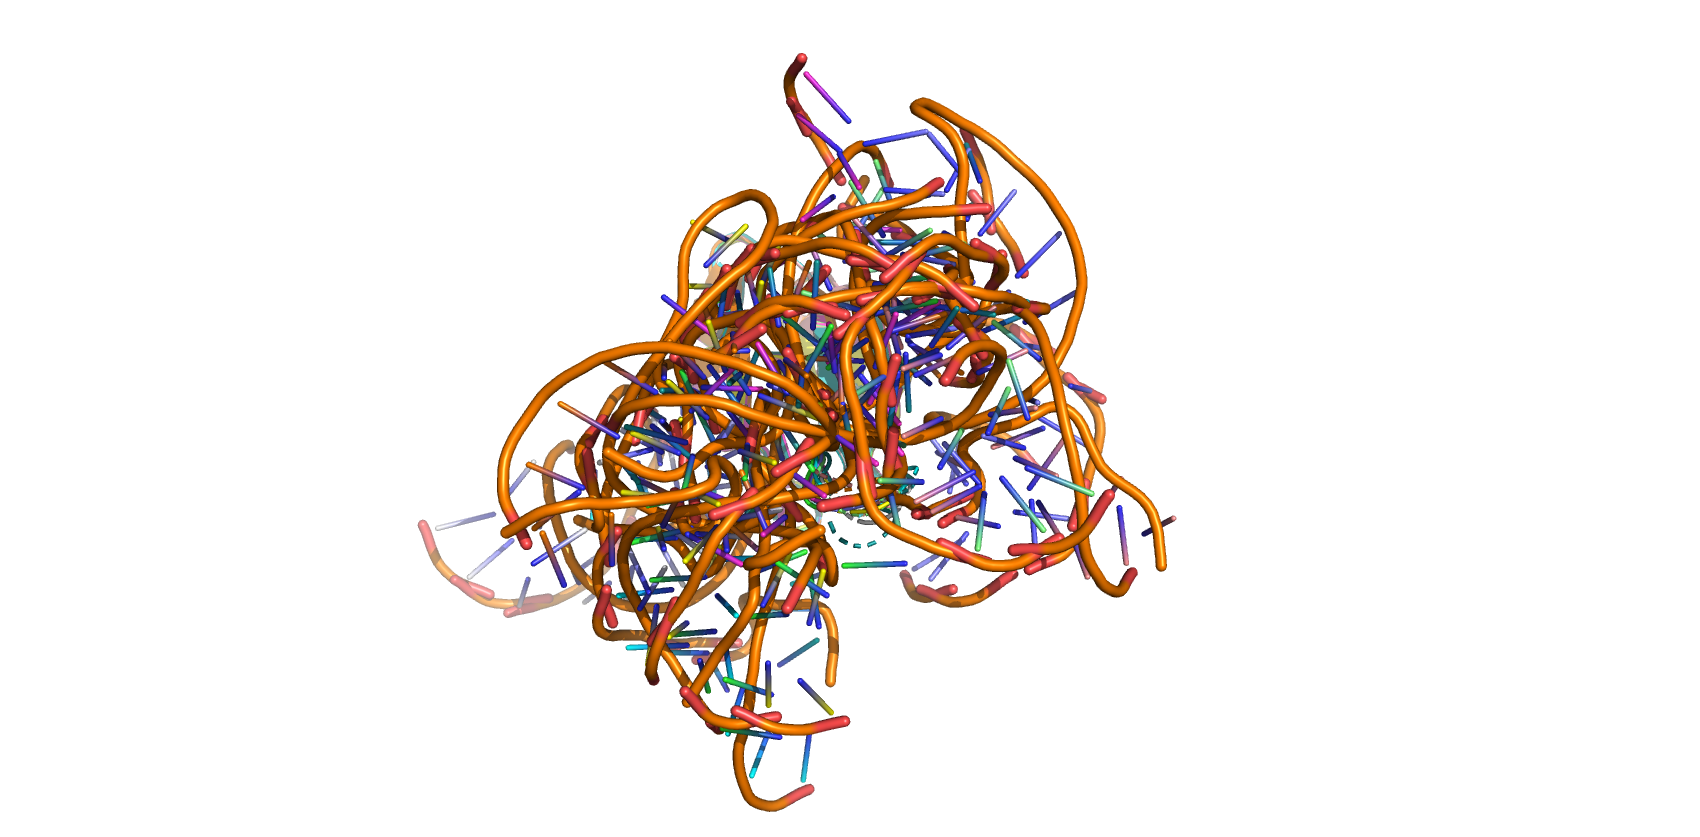
\includegraphics[width=0.9\linewidth]{assets/RMM1_mut1_ALL.png}
% \end{center}

% Podemos observar que los modelos difieren muchísimo entre sí. Parece ser que la mutación desestabiliza la interacción.  Visualizado con \href{https://pymol.org/2/}{\texttt{Pymol}}.

% \subsection*{Anexo J: Visualización de los 10 mejores modelos de docking entre MSI-1 y el RNA mutante 2}\label{anexo_J}
% \addcontentsline{toc}{subsection}{Anexo J: Visualización de los 10 mejores modelos de docking entre MSI-1 y el RNA mutante 2}

% \begin{center}
%     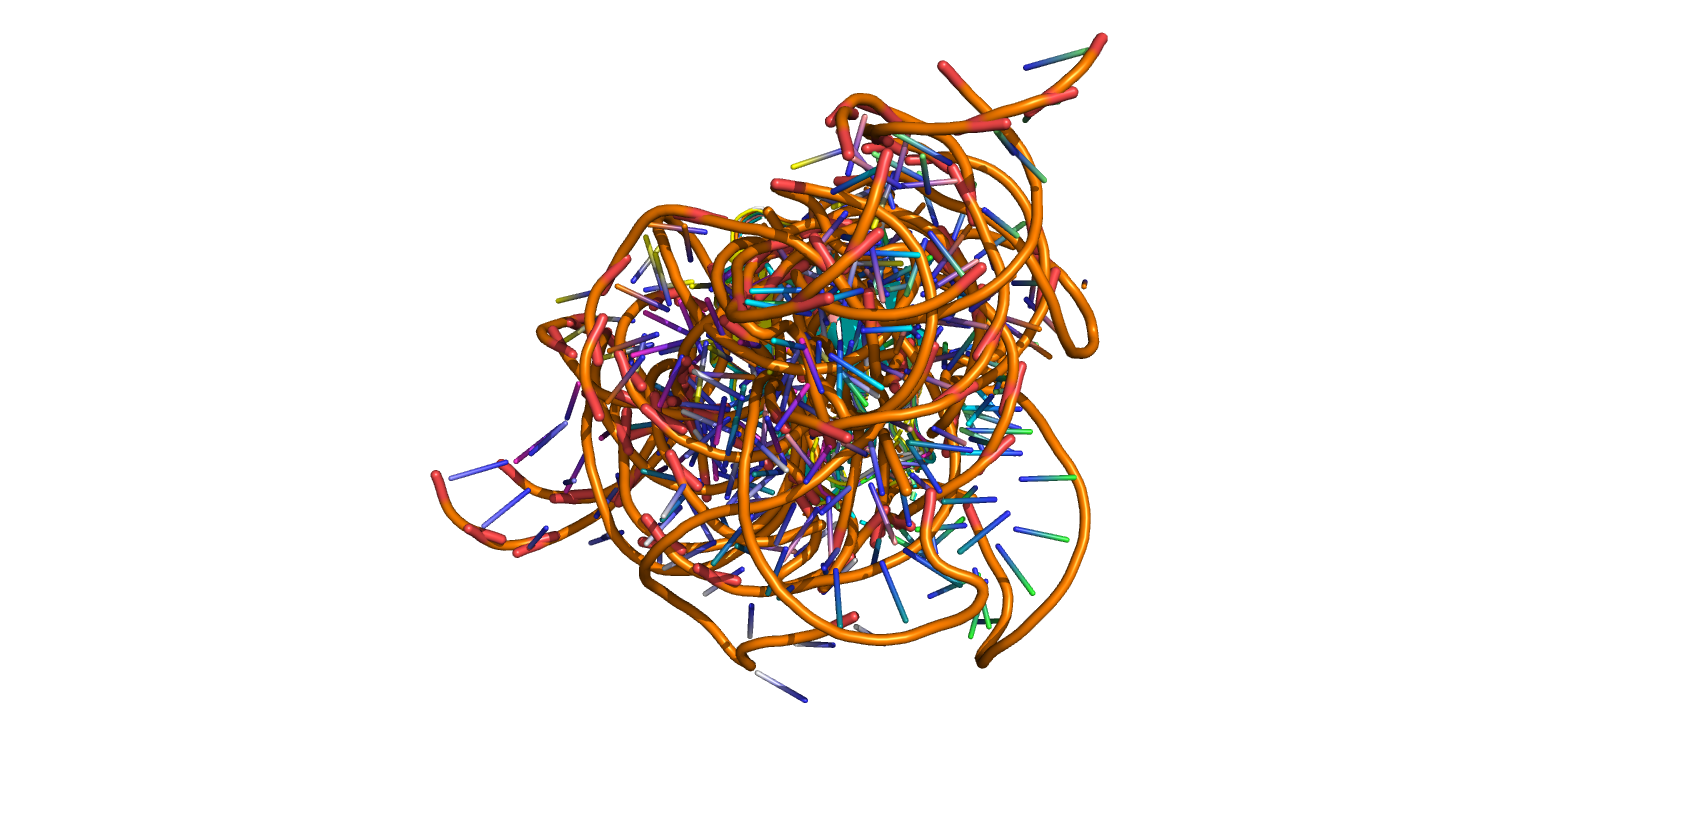
\includegraphics[width=0.9\linewidth]{assets/RMM1_mut2_ALL.png}
% \end{center}

% Podemos observar que los modelos difieren muchísimo entre sí. Parece ser que la mutación desestabiliza la interacción.  Visualizado con \href{https://pymol.org/2/}{\texttt{Pymol}}.

% \subsection*{Anexo K: Visualización de los 10 mejores modelos de docking entre MSI-1 y el RNA mutante 3}\label{anexo_K}
% \addcontentsline{toc}{subsection}{Anexo K: Visualización de los 10 mejores modelos de docking entre MSI-1 y el RNA mutante 3}

% \begin{center}
%     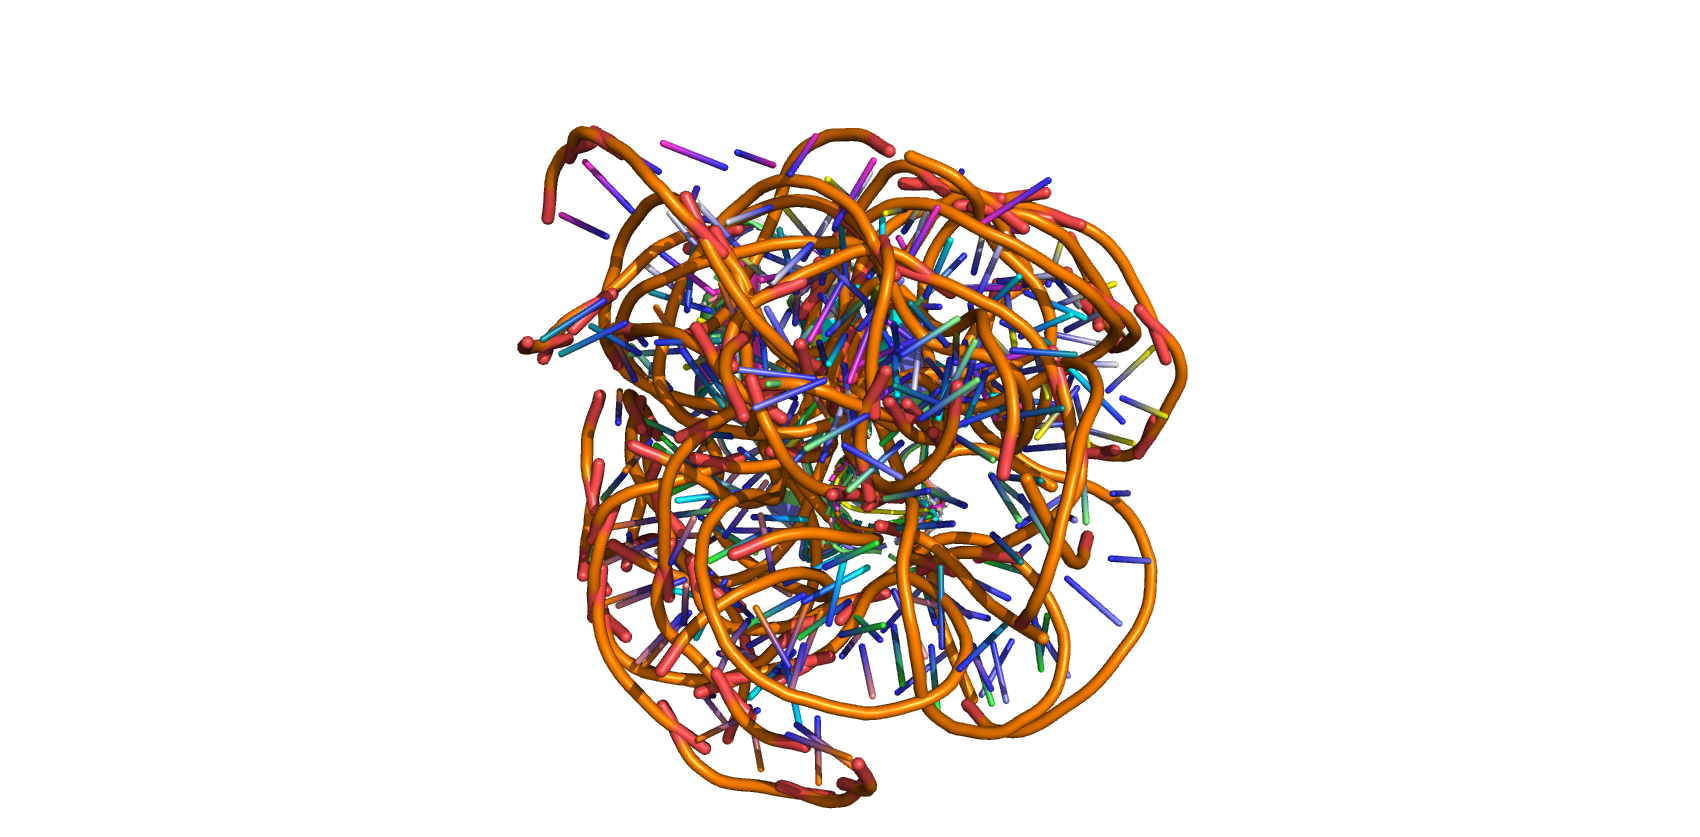
\includegraphics[width=0.9\linewidth]{assets/RMM1_mut3_ALL.png}
% \end{center}

% Podemos observar que los modelos difieren muchísimo entre sí. Parece ser que la mutación desestabiliza la interacción.  Visualizado con \href{https://pymol.org/2/}{\texttt{Pymol}}.

% \subsection*{Anexo L: Visualización de los 10 mejores modelos de docking entre MSI-1 y el RNA mutante 4}\label{anexo_L}
% \addcontentsline{toc}{subsection}{Anexo L: Visualización de los 10 mejores modelos de docking entre MSI-1 y el RNA mutante 4}

% \begin{center}
%     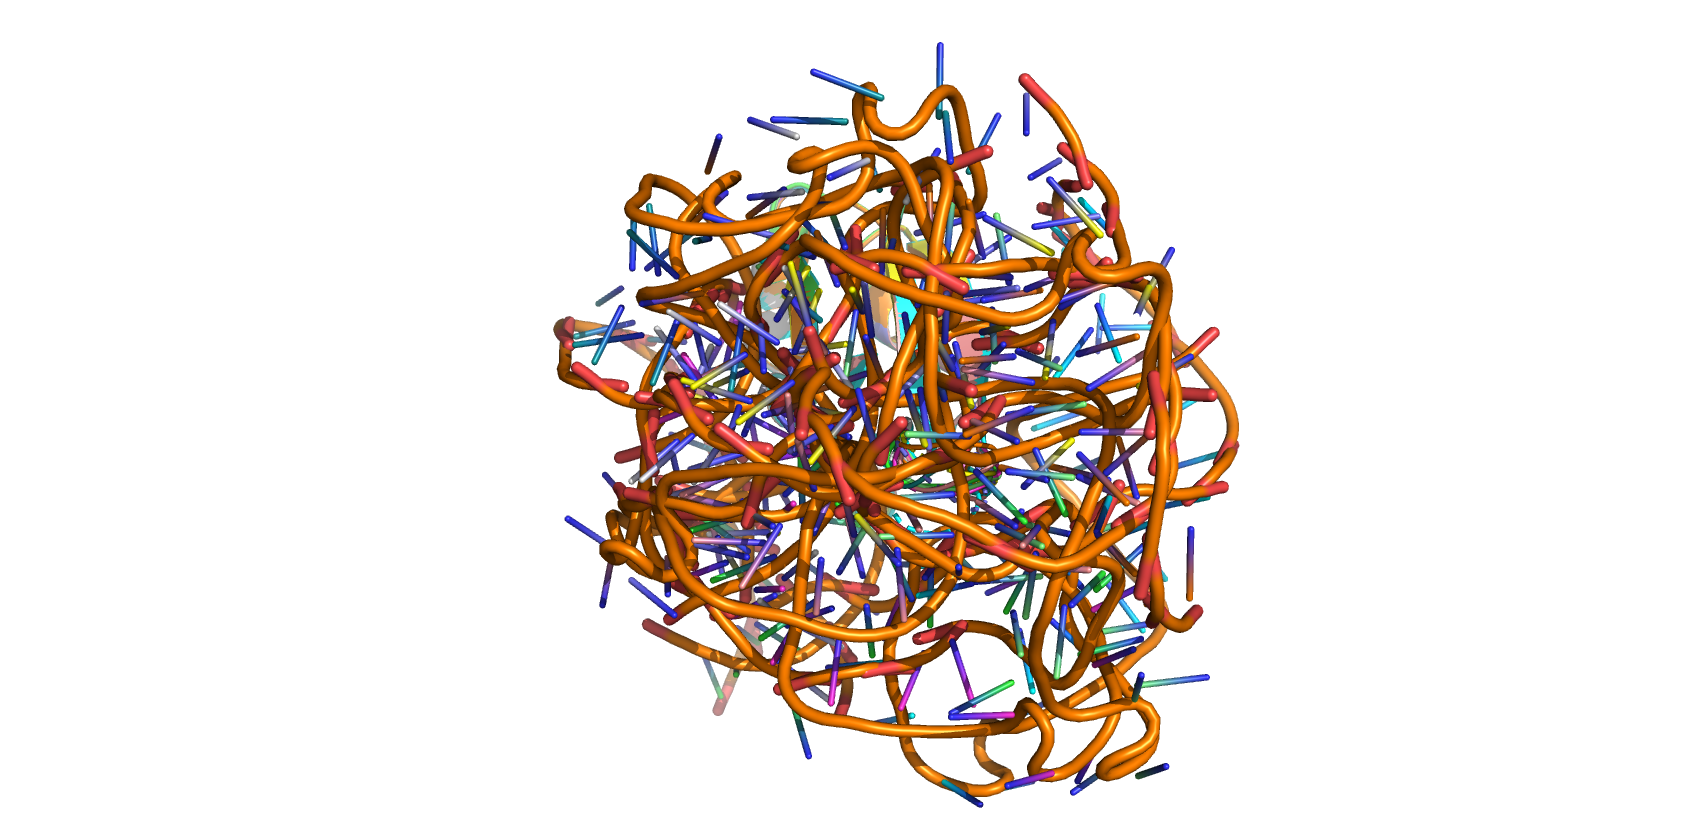
\includegraphics[width=0.9\linewidth]{assets/RMM1_mut4_ALL.png}
% \end{center}

% Podemos observar que los modelos difieren muchísimo entre sí. Parece ser que la mutación desestabiliza la interacción.  Visualizado con \href{https://pymol.org/2/}{\texttt{Pymol}}.

% \subsection*{Anexo M: Visualización de los 10 mejores modelos de docking entre MSI-1 y el RNA mutante 5}\label{anexo_M}
% \addcontentsline{toc}{subsection}{Anexo M: Visualización de los 10 mejores modelos de docking entre MSI-1 y el RNA mutante 5}

% \begin{center}
%     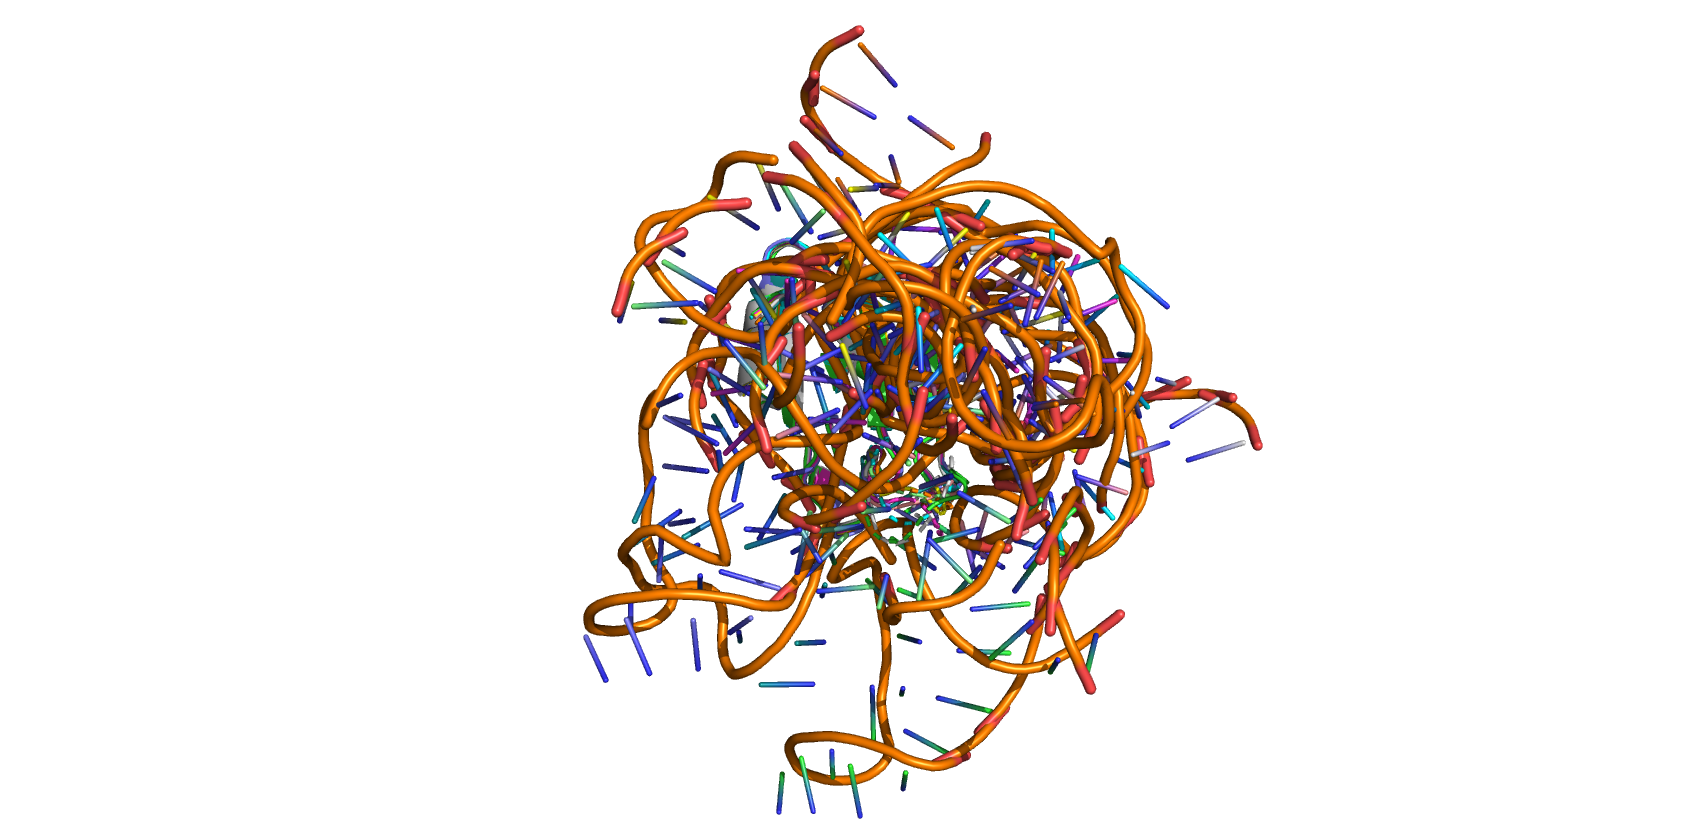
\includegraphics[width=0.9\linewidth]{assets/RMM1_mut5_ALL.png}
% \end{center}

% Podemos observar que los modelos difieren muchísimo entre sí. Parece ser que la mutación desestabiliza la interacción.  Visualizado con \href{https://pymol.org/2/}{\texttt{Pymol}}.

% \subsection*{Anexo N: Tabla de scores para los 10 mejores modelos de cada experimento de docking}\label{anexo_N}
% \addcontentsline{toc}{subsection}{Anexo N: Tabla de scores para los 10 mejores modelos de cada experimento de docking}

% \lstinputlisting{assets/allScores.table}

% \subsection*{Anexo O: Visualización de los 10 mejores modelos de docking entre MSI-1 y el RNA original en estructura lineal (sin estructura secundaria)}\label{anexo_O}
% \addcontentsline{toc}{subsection}{Anexo O: Visualización de los 10 mejores modelos de docking entre MSI-1 y el RNA original en estructura lineal (sin estructura secundaria)}

% \begin{center}
%     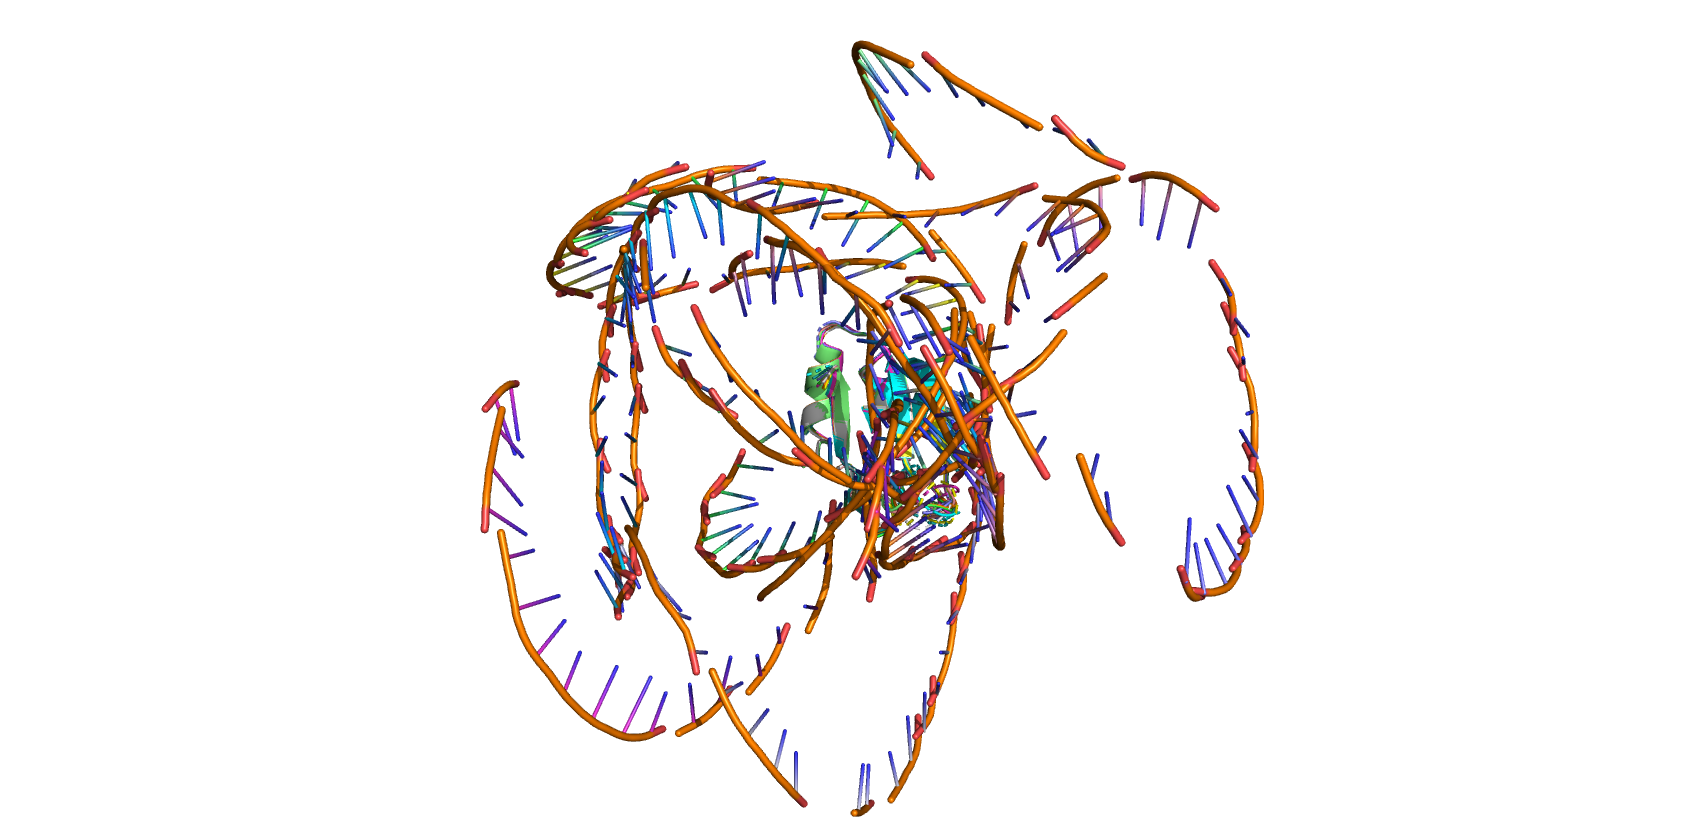
\includegraphics[width=\linewidth]{assets/linear_no_restraints.png}
% \end{center}

% Podemos observar que los modelos difieren muchísimo entre sí. En comparación con la simulación mediante el RNA con la estructura secundaria adecuada, la estructura lineal da peores resultados. Este resultado es coherente con la naturaleza, puesto que en disolución, el RNA adopta estructuras secundarias para la minimización de su energía libre de Gibbs.  Visualizado con \href{https://pymol.org/2/}{\texttt{Pymol}}.